\documentclass{sig-alternate-ipsn13}

\begin{document}

\title{Automatically Countdown Clock with Less User Manipulation}
% \title{Automatically Countdown Clock with No Greasy Hands Wash Requirement}

%
% You need the command \numberofauthors to handle the 'placement
% and alignment' of the authors beneath the title.
%
% For aesthetic reasons, we recommend 'three authors at a time'
% i.e. three 'name/affiliation blocks' be placed beneath the title.
%
% NOTE: You are NOT restricted in how many 'rows' of
% "name/affiliations" may appear. We just ask that you restrict
% the number of 'columns' to three.
%
% Because of the available 'opening page real-estate'
% we ask you to refrain from putting more than six authors
% (two rows with three columns) beneath the article title.
% More than six makes the first-page appear very cluttered indeed.
%
% Use the \alignauthor commands to handle the names
% and affiliations for an 'aesthetic maximum' of six authors.
% Add names, affiliations, addresses for
% the seventh etc. author(s) as the argument for the
% \additionalauthors command.
% These 'additional authors' will be output/set for you
% without further effort on your part as the last section in
% the body of your article BEFORE References or any Appendices.

\numberofauthors{1} %  in this sample file, there are a *total*
% of EIGHT authors. SIX appear on the 'first-page' (for formatting
% reasons) and the remaining two appear in the \additionalauthors section.
%
\author{
% You can go ahead and credit any number of authors here,
% e.g. one 'row of three' or two rows (consisting of one row of three
% and a second row of one, two or three).
%
% The command \alignauthor (no curly braces needed) should
% precede each author name, affiliation/snail-mail address and
% e-mail address. Additionally, tag each line of
% affiliation/address with \affaddr, and tag the
% e-mail address with \email.
%
% 1st. author
\alignauthor
Chun-Yen Hsu\\
       % \titlenote{Dr.~Trovato insisted his name be first.}\\
       \affaddr{Carnegie Mellon University}\\
       \affaddr{94035 Mountain View}\\
       \affaddr{California, USA}\\
       \email{chunyenh@andrew.cmu.edu}
% % 2nd. author
% \alignauthor
% G.K.M. Tobin\titlenote{The secretary disavows
% any knowledge of this author's actions.}\\
%        \affaddr{Institute for Clarity in Documentation}\\
%        \affaddr{P.O. Box 1212}\\
%        \affaddr{Dublin, Ohio 43017-6221}\\
%        \email{webmaster@marysville-ohio.com}
% % 3rd. author
% \alignauthor Lars Th{\o}rv{\"a}ld\titlenote{This author is the
% one who did all the really hard work.}\\
%        \affaddr{The Th{\o}rv{\"a}ld Group}\\
%        \affaddr{1 Th{\o}rv{\"a}ld Circle}\\
%        \affaddr{Hekla, Iceland}\\
%        \email{larst@affiliation.org}
% \and  % use '\and' if you need 'another row' of author names
% % 4th. author
% \alignauthor Lawrence P. Leipuner\\
%        \affaddr{Brookhaven Laboratories}\\
%        \affaddr{Brookhaven National Lab}\\
%        \affaddr{P.O. Box 5000}\\
%        \email{lleipuner@researchlabs.org}
% % 5th. author
% \alignauthor Sean Fogarty\\
%        \affaddr{NASA Ames Research Center}\\
%        \affaddr{Moffett Field}\\
%        \affaddr{California 94035}\\
%        \email{fogartys@amesres.org}
% % 6th. author
% \alignauthor Charles Palmer\\
%        \affaddr{Palmer Research Laboratories}\\
%        \affaddr{8600 Datapoint Drive}\\
%        \affaddr{San Antonio, Texas 78229}\\
%        \email{cpalmer@prl.com}
}
% There's nothing stopping you putting the seventh, eighth, etc.
% author on the opening page (as the 'third row') but we ask,
% for aesthetic reasons that you place these 'additional authors'
% in the \additional authors block, viz.
% \additionalauthors{Additional authors: John Smith (The Th{\o}rv{\"a}ld Group,
% email: {\texttt{jsmith@affiliation.org}}) and Julius P.~Kumquat
% (The Kumquat Consortium, email: {\texttt{jpkumquat@consortium.net}}).}
% \date{30 July 1999}
% Just remember to make sure that the TOTAL number of authors
% is the number that will appear on the first page PLUS the
% number that will appear in the \additionalauthors section.

\maketitle
\begin{abstract}
We design an automatically and intuitive countdown clock in order to provide user a less manipulation interface not only lessons usage interruption but also increases working efficiency to users' original work.

\end{abstract}

\section{Introduction}

% Countdown clock 1. 方便 2. 可以選擇時間按下開始後計時 3. 
% However//在某些限制多的環境下不需要
% 1. not oil protected
% 2. too much manipulation
% We present
% 在廚房內如果需要為了接觸電子器材而一直洗手將使人感到厭煩且煮飯的效率會大大降低
% 簡單操作介面
Countdown clock provides the time choice function for users to select how long times we want to count. After the time is decided, we can press the "Start" button then the clock start counting down the time. However, under some restrictive circumstances, such as cooking with greasy hands and tight cooking time slot, or doing heavy metal lab experiments which requires highly concentration to the work, too many manipulations or buttons would decrease users' efficiency and concentration to their original work. 
Besides, grease or heavy metal ingredients on our hand would let us feel anguished to touch expensive clock devices, such as our smartphone. 

We present an intuitive countdown clock(Figure \ref{fig:demo1}A), which lessons the manipulation to only one button for adding one minute in each operation and start count the time instantly. We simplify clock's user interface and operation methods in order to provide an intuitive manipulation to the clock. Also, Whenever user presses the button with a view to adding the time, the countdown clock will start counting time automatically with no additional "Start" button requirement. When time is up, the LCD display will glisten four times(Figure \ref{fig:demo1}B) to give user some reminders. In addition, with this countdown clock, user can not touch their expensive electronic clock devices anymore, such as personal mobile phone.
% provides highly surface protection to against various threat and potential notorious ingredient from users' hands. 

% 重複又無意義的動作使人厭煩, 工作

\section{Evaluation and Limitation}
We recruited 3 participants for our user study and found out that the most important factor for using countdown clock under restrictive circumstances is to let user feel convenient and comfortable. Moreover, one minute as each unit for button pressed is not too many and not too less in most cases. Besides, users seldom have to count an unique time slot, such as 23 seconds.

% \section{Limitation}
With our team members' irrelevant background and the first time for us to play with hardware, we must has several technical restriction for us to implement a countdown clock. However, We still do our best to figure out the technical skills, such as how does Arduino board work, how and why to connect the port to LCD board, and why pressing the button can give different feedback.
% to not only spend times but fix as well as figure out bugs about how hardware assemblies and principles.

% \begin{figure}
% \centering
% 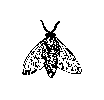
\epsfig{file=fly.eps}
% \caption{A sample black and white graphic (.eps format).}
% \label{fig:example}
% \end{figure}

\begin{figure}
  \centering
  \includegraphics[width=0.9\linewidth]{Figures/demo_big.pdf}
  \caption{(A) Intuitive Coundown Clock (B) Clock glistens while time out}
  \label{fig:demo1}
\end{figure}

\section{Conclusions}
Our product provides a single button manipulation not only simplify the operation interface but it also start counting clock automatically, which can significantly reduce the interruption and provide less manipulations to users while they are working with various environment restriction.
% Users may face various restriction while using count down clock in their daily life. However, people still require a countdown clock to help them not merely calculate the time, but also provide them a convenient user interface with less manipulations and few interruption to their original work. 
It is no doubt that the automatically countdown clock produces a great enlightenment that gives an innovative journey and new manufactured direction to the countdown clock in the market.


%ACKNOWLEDGMENTS are optional
% \section*{Acknowledgments}
% Acknowledgement goes here.

%
% The following two commands are all you need in the
% initial runs of your .tex file to
% produce the bibliography for the citations in your paper.

% %Reference
% \bibliographystyle{abbrv}
% \bibliography{sigproc}  % sigproc.bib is the name of the Bibliography in this case

% You must have a proper ".bib" file
%  and remember to run:
% latex bibtex latex latex
% to resolve all references
%
% ACM needs 'a single self-contained file'!
%
%APPENDICES are optional
%\balancecolumns
% \appendix
%Appendix A

% Appendix goes here.

% That's all folks!
\end{document}
